
\chapter{Object detection}
\label{objectDetection}

% ===========================================================================================

% ===========================================================================================

\section{Image pre-processing}
\label{imagePreprocessing}
Neural networks used for object detection are usually trained on image data that has been pre-processed, meaning the image data was converted to a supported format, resized, normalized, etc. The reason for this is that neural networks trained on pre-processed image data are usually more stable, and models can "focus" on learning objects instead of learning the brightness and color saturation of objects under different lighting conditions for a given object \cite{glossaryImagePreprocessing}.

\begin{figure}[hbt]
	\centering
	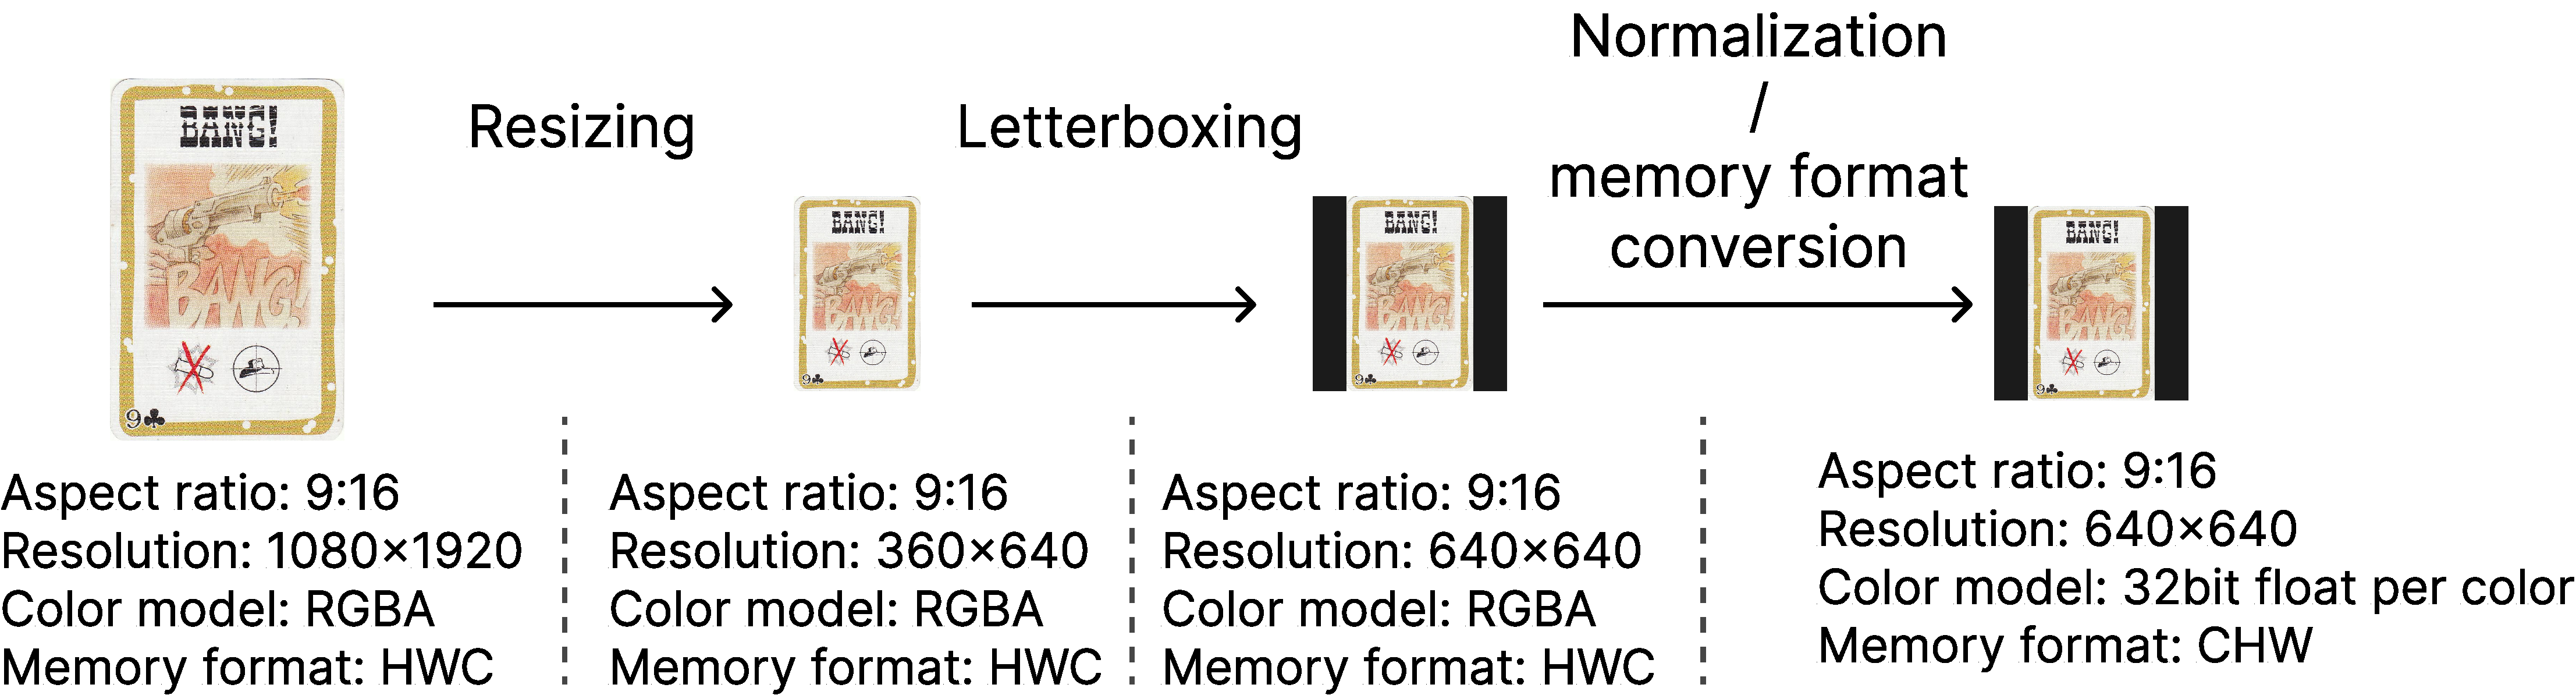
\includegraphics[width=0.98\textwidth]{obrazky-figures/preprocessing.pdf}
	\caption[Pre-processing step]{Pre-processing steps shown on scan of the Bang! card from the game Bang!.}
	\label{preprocessingFigure}
\end{figure}

When passing image data into the neural networks, it is beneficial for the data to be pre-processed in the same way as it was during its training to achieve better results. 

\subsection{Letter-boxing and resizing}
\label{letterboxing}
Some object detection models need a fixed resolution in order to perform object detection tasks. However, the image data provided by the camera might not always be in the correct resolution, therefore, rescaling is needed \cite{letterboxingAndNormalization}.

For example, the camera provides an image with\texttt{1920x1080} resolution in portrait mode. The model requires an image with a resolution of \texttt{640x640}. Rescaling the image would create a \texttt{640x640} image; however, the original aspect ratio of the image was \texttt{16:9} or \texttt{9:16} in portrait mode. This would be changed to a \texttt{1:1} aspect ratio. This distortion could affect object detection.

Instead, resize the image using the larger dimension and use that to scale the image. However, the resolution of that image would be \texttt{640x360}, which means that only one of the dimensions will satisfy the resolution required by the model. To fix that, letter-boxing is introduced, and the dimension that does not satisfy the required resolution will be padded with a default value, resulting in a final image size of \texttt{640x640}. This ensures the image has the correct resolution and is not distorted.


\subsection{Normalization and representing colors in a image}
Images can be represented as a matrix or a 2-dimensional array of pixels, where each pixel is represented by three values: red, green, and blue. This format is also known as RGB. These values are usually unsigned integers with 8 bits per color, resulting in the 8 bit RGB format. However, neural networks are mostly trained on normalized float values. Each color channel is converted into a float and normalized by the value \texttt{255}, which is the highest possible value the 8 bit channel can achieve.


\subsection{Converting colors channel formats}
The section above explained different ways of storing each pixel as a set of values, whether it was 3 sets of 8 bit integers per pixel or 3 sets of float values per pixel. However, there are also formats that change how these pixels are stored in memory. Probably the most commonly used and intuitive way of storing image data is to imagine that the image is a matrix with width and height, or height and width. Now, each element of this matrix could be a pixel; therefore, we are dealing with a 2D matrix of pixels. This is called \textbf{HWC} format: Height x Width x Channel, where the channel refers to all available color channels. For RGB, there would be three channels, and for RGBA (with A at the end representing alpha, allowing pixels to be semi-transparent or fully transparent).

The other format commonly used in neural networks, especially those aimed at image processing, is \textbf{CHW}, Channel X Height x Width. This is different from the \textbf{HWC} format; instead of having a 2D matrix of pixels, each containing 3 colors (considering that the image is coded in 3 color channels: Red, Green, and Blue), the format uses 3 separate channels, each containing color values in a 2D matrix \cite{channelFormatsIntel} \cite{channelFormatsSynopsis}. This format is beneficial for GPUs and NPUs as it is more suited for the kind of operations  they perform, especially parallel and vector operations \cite{chwAndHwcFormats}. Simple example of memory arrangement for these two formats for images with 3 color channels for 2x2 image:

\begin{verbatim}
HWC
r0, g0, b0, r1, g1, b1, r2, g2, b2, r3, g3, b3

CHW
r0, r1, r2, r3, g0, g1, g2, g3, b0, b1, b2, b3
\end{verbatim}

Neural networks that were trained on data in \textbf{CHW} format will also expect this format during inference runs, meaning all image data used for object detection by the neural network must be converted to this format as well.

\begin{figure}[hbt]
	\centering
	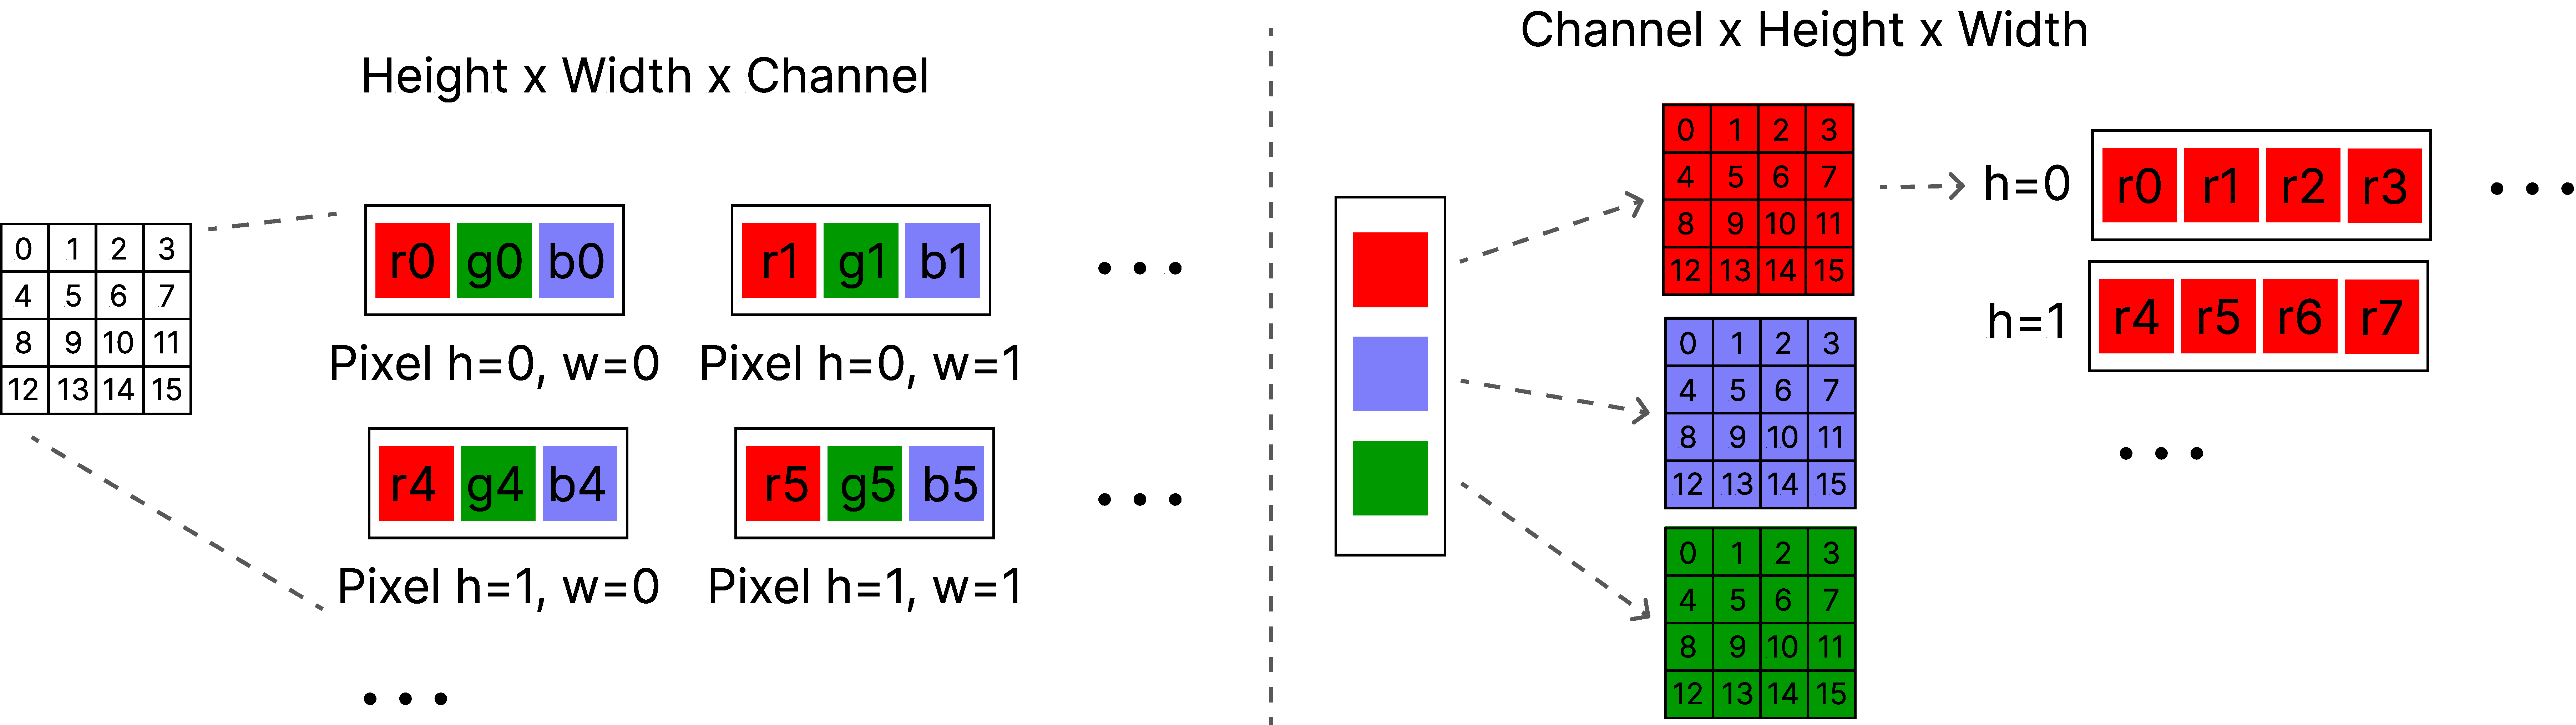
\includegraphics[width=0.98\textwidth]{obrazky-figures/channels.pdf}
	\caption[Image memory data layout of HWC and CHW]{Figure showing difference between HWC on the left, and CHW on the right. Both show 4x4 image with 3 color channels.}
	\label{ChannelsFigure}
\end{figure}

% ===========================================================================================

% ===========================================================================================

\section{Post-processing}
After pre-processing, the image was transformed into a suitable format that is usable by the neural network. The results of this inference run are further processed. This step is called \textbf{post-processing}, and its purpose is to extract usually raw float values into more structured data, finally resulting in final sets of detections. 

\subsection{Data extraction}
The first step is to extract the data from the output type of the inference engine into a more developer-friendly array style. Both \texttt{YoloOnnxDetector} and \texttt{YoloOpenCVDetector} have different types of outputs. However, both of these \texttt{Detectors} outputs can be converted to a 1-dimensional array of float values.

In order to extract values, it is necessary to know the layout of the data, which for YOLO neural networks converted to ONNX format is: \texttt{[batch]x[attributes]x[detections]}. Where the \textbf{batch} is always 1 because \texttt{Detectors} work with only a single image; therefore, the shape is effectively \texttt{[attributes]x[detections]}. The \textbf{attributes} are individual values from the detection, meaning: x, y, width, height, and confidence score of each class. \textbf{Detections} refer to the number of detections.

\begin{figure}[hbt]
	\centering
	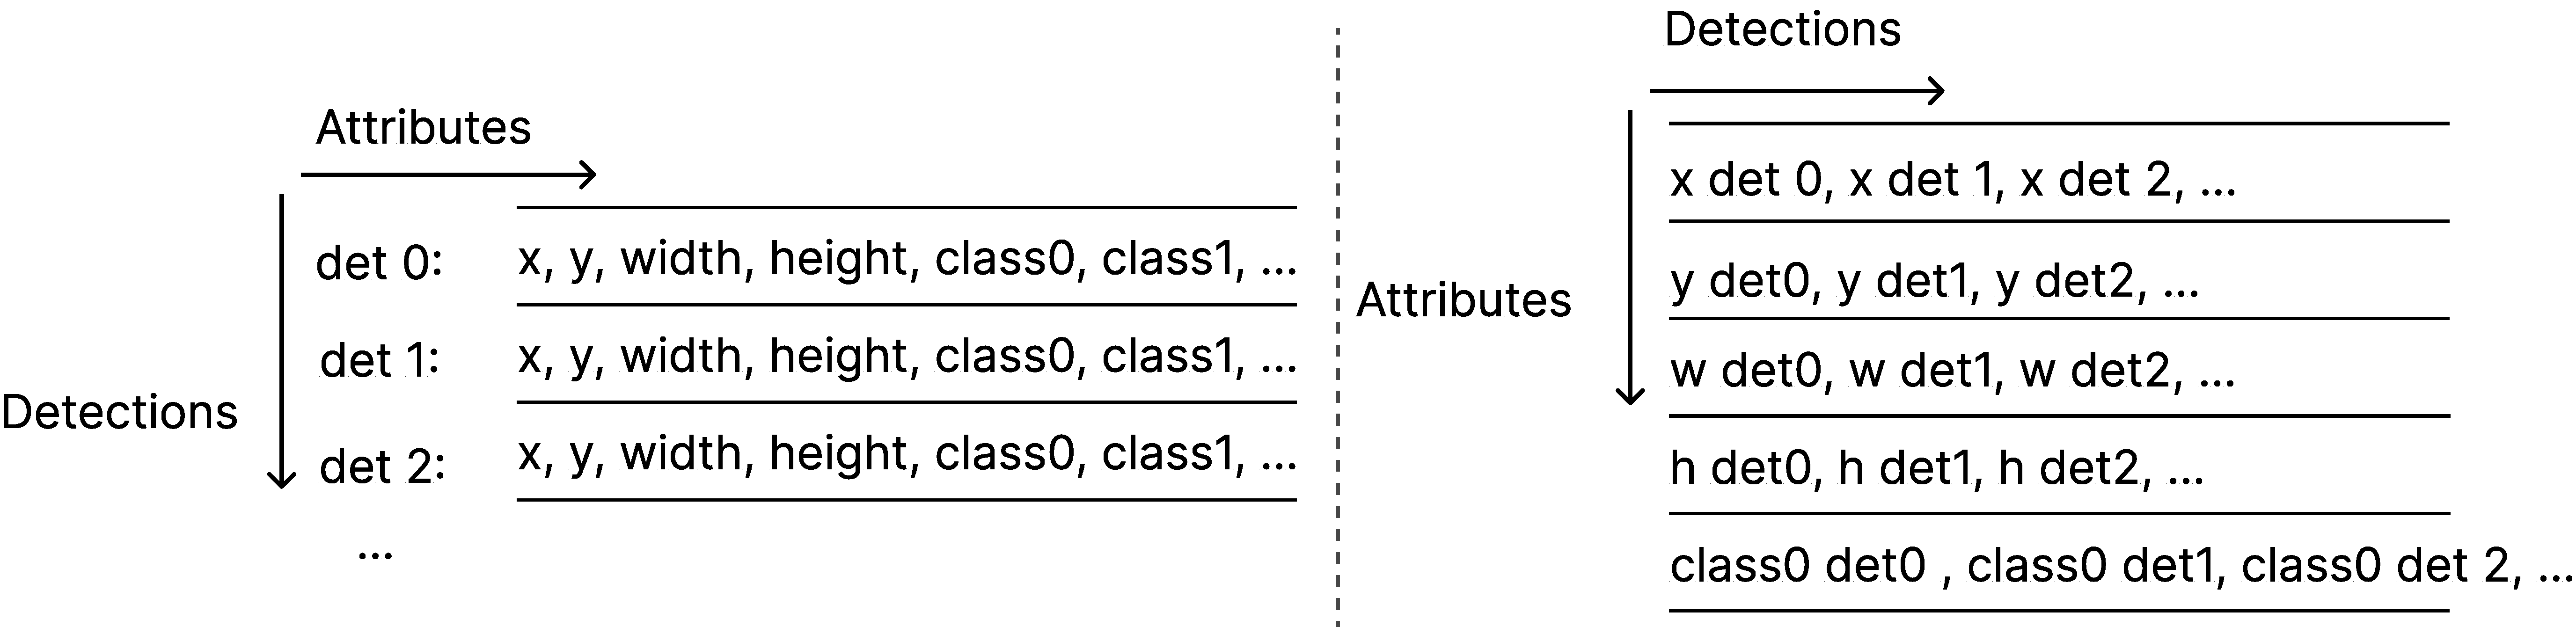
\includegraphics[width=0.98\textwidth]{obrazky-figures/extracted_data_layout.pdf}
	\caption[Memory layout of raw extracted detections]{Figure showing data layout in memory, on the left [detections]x[attributes], on the right [attributes]x[detections].}
	\label{ExtractedDataLayoutFigure}
\end{figure}

However, the \texttt{[attributes]x[detections]} shape might not be the most intuitive one. Therefore, there are two options: use it as it is or transpose the data. Both are valid options, and in mathematics, transposing might be preferred. However, in computer science, operations such as these take time. In code, these operations mean allocating new arrays and copying data into them.

\begin{verbatim}
// data : array containing data in [attributes]x[detections] format 
for(column in 0 until numberOfDetections) {
    val x = data[0 * numberOfDetection + column]
    val y = data[1 * numberOfDetection + column]
    // ...
}    
\end{verbatim}

\begin{verbatim}
// data : array containing data in [detections]x[attributes] format 
for(attributes in data) {
    val x = attributes[0]
    val y = attributes[1]
    // ...
}    
\end{verbatim}

The abstract code snippet above shows the difference between the two approaches. A very simple test for both of these methods shows that transposing the data is 3 times slower, which is approximately \texttt{5.18 milliseconds}. Therefore, a direct approach mirroring the memory layout was chosen as the final solution for both included \texttt{Detectors}.

\textit{Note: all of the above mentioned data were collected using the YOLOv8 model and on an available device whose hardware capabilities are mentioned in \ref{bangTrainingExperiments}.}

Lastly, it is necessary to determine the best class with the highest confidence score. This is done by retrieving all confidence scores and simply remembering the highest value and the index.

\begin{verbatim}
var bestClass : Int = -1
var bestScore : Float = 0f

for (row in 4 until numOfAttributes) {
    val score = data[row * numOfDetections + column]
    if (score > bestScore) {
        bestClass = row - 4
        bestScore = score
    }
}
\end{verbatim}

\subsection{Thresholding and Non-Maximum Suppression}
The result of the extraction step is a list of \texttt{Detection} (see \ref{DetectionClass}) objects. Each object contains x and y coordinates, height and width dimensions, and its best class and confidence score. However, before creating an object, the best confidence score is checked. If the value of the score is above the \textbf{threshold} value, an object will be created; otherwise, this detection will be skipped.

\subsubsection{Non-Maximum Suppression}
The object detection model might output multiple bounding boxes for one object. These duplications need to be removed, and the most proven method is \textbf{Non-Maximum Suppression} \cite{nms}. If the computed \textbf{Intersection Over Union} or \textbf{IoU} for two detections is past a threshold, the detection with the lower confidence score is removed. The NMS algorithm can be simplified into 3 steps \cite{nms}:

\begin{enumerate}
  \item {Choose the detection with the highest confidence score from all detections, remove it from the list of all detections, and add it to the list of kept ones.}
  
  \item {Compute IoU for the chosen detection and the rest of the detections. If the IoU for the detection from the list of all detections is above the threshold, remove it from the list of all detections.}
  
  \item {Repeat until the list of all detections is empty.}
\end{enumerate}

The code below shows the implementation of NMS. The list of detections is sorted by score at the start instead of looking for the best score in each step. It should be noted that this code does not work and is not used, as deleting an item from the list while iterating it  will result in an error. Instead, a method with boolean masks is applied to detections that should be removed and are skipped instead. However, this version is more straightforward and better for illustrating the NMS algorithm.

\begin{verbatim}
detections.sortByDescending { it.score }
keptDetections = mutableListOf<Detection>()
while (detections.isNotEmpty()) {
    val best = detections.first()
    keptDetections.add(best)
    detections.remove(best)

    // check all other detections, remove ones with IoU > threshhold
    for (detection in detections) {
        val iou = computeIoU(best, detection)

        if (iou > threshold)
            detections.remove(detection)
    }
}
\end{verbatim}

\begin{figure}[hbt]
	\centering
	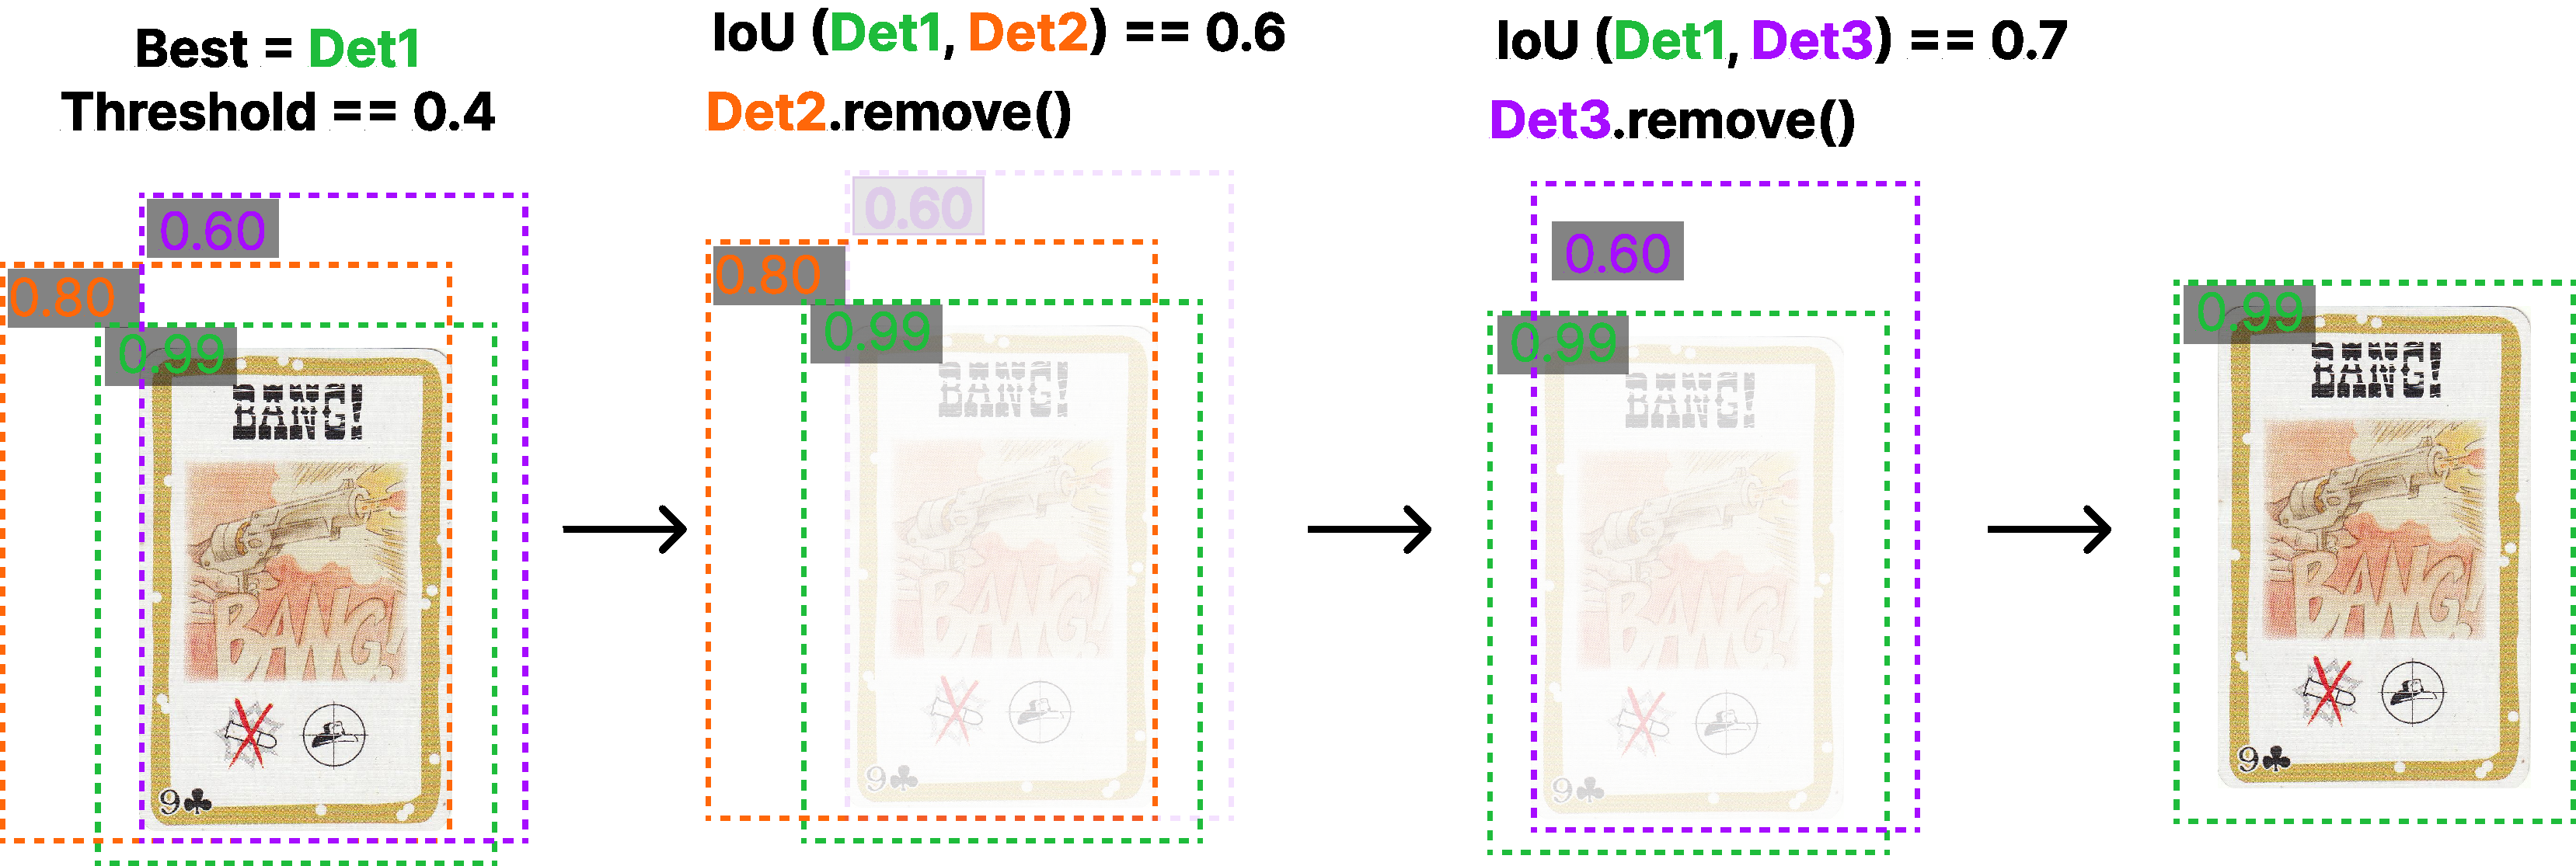
\includegraphics[width=0.90\textwidth]{obrazky-figures/nms_example.pdf}
	\caption{Simplified Non-Maximum Suppression demonstration.}
	\label{nsmDemonstration}
\end{figure}

This, however, can result in other classes deleting other classes; for example, a human holding an apple, where the apple might be deleted because it is overlapping with the human. Because of that, NMS is on grouped classes; therefore, only the human class can remove the human class.

\textbf{CV.ILIBG} also contains another implementation of NMS that uses OpenCV's built in NMS filtering method. However, this method requires converting the \texttt{Detection} objects into OpenCV's \texttt{Rect2D} objects. This method is \texttt{1.5} to \texttt{2} times slower, with a time difference of 63 nanoseconds, compared to the method written in Kotlin using \texttt{Detection} objects.

NMS is not a cheap operation as it has to iterate through all detected objects multiple times. Therefore, it is recommended to first reduce the number of detections with thresholding or other methods \cite{nms2}. Lastly, NMS can use confidence softening instead of removing detections. However, this approach is usually not used for real-time detection tasks. 